
\documentclass[11pt, oneside]{article}

\usepackage[a4paper, tmargin=30mm, bmargin=30mm]{geometry}
\usepackage{graphicx}
\usepackage{xcolor}
\usepackage{enumerate}	
\usepackage{amsmath}
\usepackage{amssymb,mathrsfs}
\usepackage{parskip}

\newcounter{thmcount}
\renewcommand{\thethmcount}{\arabic{thmcount}}

\newtheorem{thm}[thmcount]{Theorem}
\newtheorem{cor}[thmcount]{Corollary}
\newtheorem{prop}[thmcount]{Proposition}

\def\X{\mathcal{X}}
\def\P{\mathcal{P}}
\def\U{\mathcal{U}}
\def\V{\mathcal{V}}
\def\W{\mathcal{W}}
\def\Y{\mathcal{Y}}

\def\R{\mathbb{R}}
\def\B{\mathscr{B}}

\def\conv{\mathrm{conv}}
\begin{document}

% Define $c_1 = c_1(\varrho)$, $P = P(\varrho)$ and 
% $\varrho = \arg\max_{r} (1-r) c_1(r)$, where $c_1(r) = 1/\sqrt{t(r)}$ and $t(r)$, $P(r)$ are defined for any given $r\in(\rho(\Psi),1)$ by
% \[
% \bigl(t(r),P(r)\bigr) 
% = \arg\min_{t,P}\ t \ \ \text{subject to} \ \
% r^2 P \succ \Psi^T P \Psi \ \ \text{and} \ \
% \begin{bmatrix} t & \xi_j^T \\ \xi_j & P\end{bmatrix} \succ 0 \ \forall j\in\mathbb N_r ,
% \]
% which requires solution of a semidefinite program. The optimal value of $\varrho$ (and hence $c_1(\varrho)$ and $P(\varrho)$) can be determined by performing a line-search over $r\in(\rho(\Psi),1)$ to find the maximizer of $(1-r)c_1(r)$.
%

We need to determine $c_1,c_2,c_3$, $P$ and $\varrho$ so that:
\begin{subequations}\label{eq:constr1}
\begin{align}
& P \succ 0  , \quad \varrho^2 P \succ \Psi^T P \Psi \\
& \B_P(c_1) \subseteq \X \\
& \B_P(c_2) \supseteq \P_n \\
& \B_P(c_3) \supseteq \V(x) \ \ \forall x \in \X
\end{align}
\end{subequations}
and we additionally require that $c_1 > (1-\varrho)^{-1}c_3$ holds whenever this is possible.

$\rule{7pt}{7pt}$\hspace{1ex}
Note that $\varrho$ must lie in the interval $[\rho(\Psi),1)$ and that 
$c_2$ can be determined for given $P$ and $\varrho$ as $c_2 = \max_j \|x_j\|_P$, where $\conv_j \{ x_j \} = \P_n$.

$\rule{7pt}{7pt}$\hspace{1ex}
The problem of determining $c_1,c_3$, $P$ and $\varrho$ is under-constrained (because an arbitrary scaling of $P$ can be absorbed in the values of $c_1,c_3$); hence there is no loss of generality in setting $c_1 =1$.

$\rule{7pt}{7pt}$\hspace{1ex}
We would like to determine $c_1, c_3$, $P$ and $\varrho$ by solving a optimization which ensures that $c_1 > (1-\varrho)^{-1}c_3$, whenever this is possible. For example, setting $c_1=1$, the minimizer of $(1-\varrho)^{-1}c_3$ subject to (\ref{eq:constr1}a,b,d) has this property.

However the constraint $\varrho^2 P \succ \Psi^T P \Psi$ cannot be expressed as a convex condition on $\rho$ and $P$ (or transformations of these variables). 

Therefore consider the (non-convex) problem of minimizing $(1-\varrho)^{-1}c_3(\varrho)$ via a linesearch over $\varrho\in [\rho(\Psi),1)$, where $c_3(\varrho)$ and $P(\varrho)$ are defined by the solution of a convex problem:
\[
\bigl( c_3^2(\varrho), P(\varrho) \bigr) = \arg\min_{c_3^2,P}\ c_3^2 \ \ \text{subject to} \ \
\begin{aligned}[t]
& P \succ 0,  \ \ \varrho^2 P - \Psi^T P \Psi \succ 0\\
& P \succeq \Xi_j \Xi_j^T \quad \forall j \\
& c_3^2 \geq v_k^T P v_k \quad \forall k
% & \begin{bmatrix} \Theta & \Xi \\ \Xi^T & P \end{bmatrix} \succeq 0 ,\ \Theta_{jj} \leq 1 \forall j
\end{aligned}
\]
where 
$\{x: \Xi x \leq {\bf 1}\} = \X$, and where 
$\conv_k \{ v_k \}$ has the property that
$\V(x) \subseteq \conv_k \{ v_k\}$ for all $x\in \X$, and for all $v \in \conv_k \{ v_k\}$ there exists $x\in\X$ such that $v\in\V(x)$.

For an example with randomly chosen $\Psi$, $\Xi$ and $\conv_k\{ v_k\}$ the solution is shown below.

\centerline{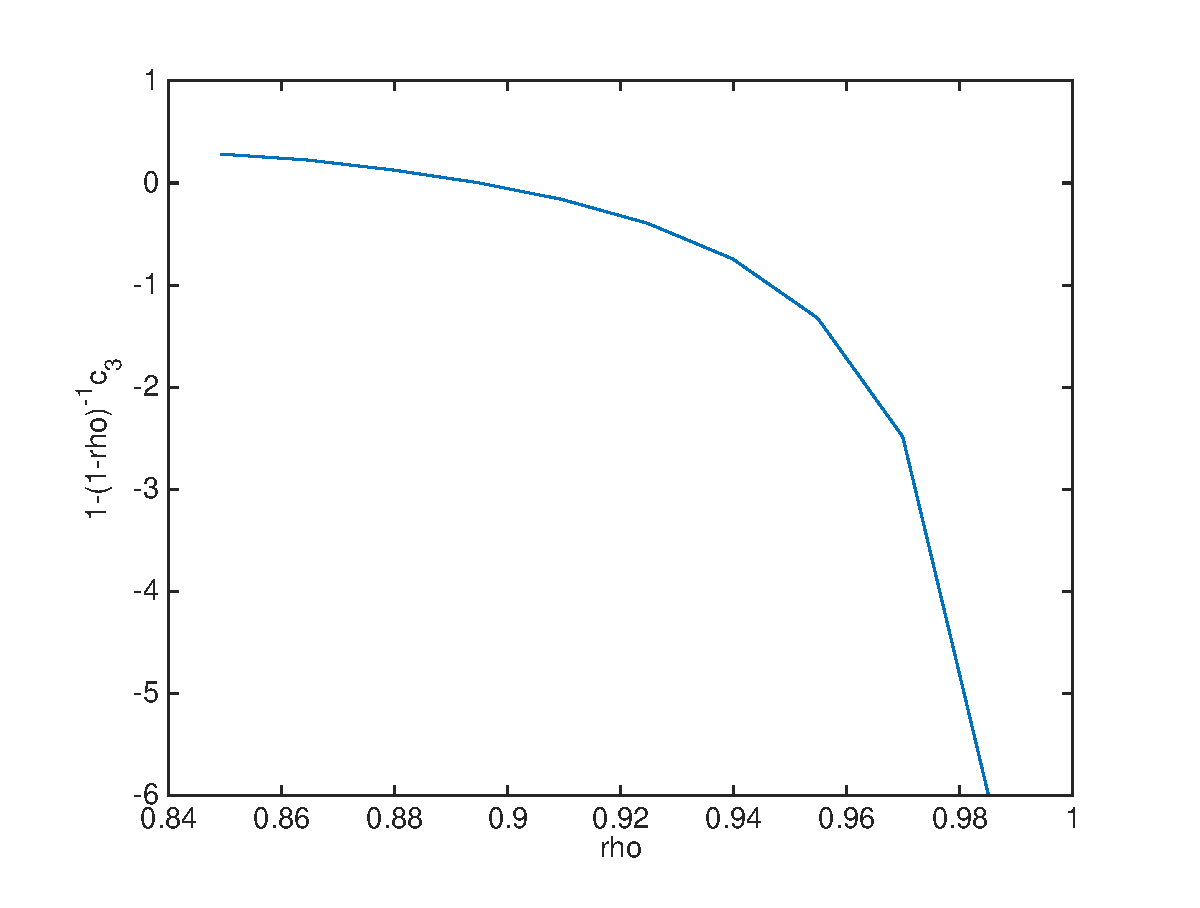
\includegraphics[scale=0.5]{./tmp/obj_rho}
\hspace{-10mm}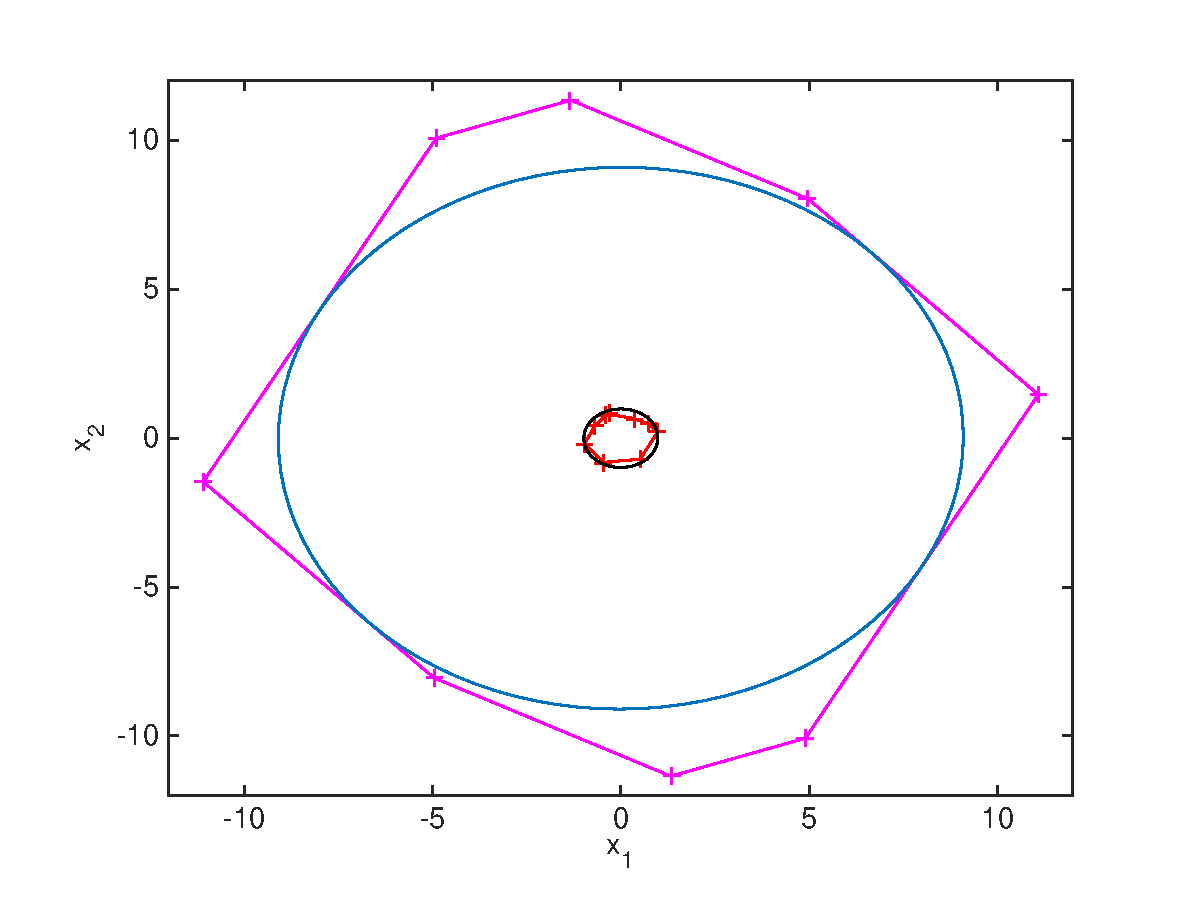
\includegraphics[scale=0.5]{./tmp/sets}}

Left: $1 - (1-\varrho)^{-1}c_3(\varrho)$ as a function of $\varrho$; for $\rho \in [0.85, 0.895]$ we get $1 - (1-\varrho)^{-1}c_3(\varrho) > 0$, and the minimizer of $(1-\varrho)^{-1}c_3(\varrho) $ is $\varrho = \rho(\Psi) = 0.85$. Right: the sets $\X$ (pink), $\B_P(1)$ (blue), $\conv_k \{ v_k \}$ (red) and $\B_P(c_3)$ (black) for $\rho=0.85$.


\end{document}